\chapter{Pré-requis et installation}
\label{chap-setup}

\renewcommand{\headrulewidth}{0.3pt} 
\fancyhead[LE]{\thepage} 
\fancyhead[RE]{\nouppercase{\textbf{\leftmark}}}
\fancyhead[RO]{\thepage} 
\fancyhead[LO]{\nouppercase{\textbf{\rightmark}}}
\fancyfoot[L,C,R]{}

\setlength{\parindent}{0.35cm} 

\minitoc
\newpage \ \newpage  

% ================================================================

Le plug-in \cwv~a été conçu pour fonctionner sous le système d'information géographique (SIG) QGIS. Il a initialement été développé sous QGIS 3.28\footnote{Disponible à l'adresse : \href{https://www.qgis.org/fr/site/forusers/download.html}{https://www.qgis.org/fr/site/forusers/download.html}}, et utilisé actuellement sous sa version 3.36. Son bon fonctionnement n'est pas garanti pour une utilisation sous version ultérieure. 

\section{Installation des dépendances} \label{setup-dependances}
Dans sa première version, \cwv~ne propose pas encore d'installateur de dépendances. Il sera donc nécessaire de les installer préalablement à l'installation de \cwv. 

\subsection{Installation sous Microsoft Windows} \label{setup-windows}

L'installation des dépendances sous Microsoft Windows est plus simple à réaliser directement à l'aide de l'interpréteur Python, intégré à QGIS. À cet effet, ouvrir une console Python\footnote{En cliquant sur 
\includegraphics[height=0.45cm]{1_installation_requirements/fig/interpreteur_python.png} dans l'interface QGIS.}
 et taper les commandes suivantes :  

\begin{lstlisting}[language=python]
>>> import pip
>>> pip.main(['install', 'pandas', 'numpy', 'ipython', 'matplotlib', 'geopandas'])
\end{lstlisting} 

\alertinfo{L'installation des dépendances depuis un autre interpréteur Python que celui utilisé par votre version de QGIS ne permettra pas à ce dernier d'accéder aux librairies nécessaires au plug-in. Veillez donc à installer les dépendances nécessaires depuis l'interpréteur python interne à QGIS.}

\subsection{Installation sous distribution Linux} \label{setup-linux}
L'installation des dépendances sous distribution Linux est réalisée à partir du terminal de commande. Veillez à installer les dépendances suivantes : pandas, numpy ipython, matplotlib, geopandas.



\section{Installation classique du plug-in (utilisateurs)} \label{sec-install-user}

L'installation du plug-in se fait \textit{via} QGIS, en important l'archive de plug-in (\script{.zip}), téléchargée préalablement depuis le dépôt GitLab (\href{https://gitlab.com/gviz/cawaqsviz}{https://gitlab.com/gviz/cawaqsviz}) de l'extension (\cref{fig-download_cwv}). Une fois téléchargée, ouvrez QGIS.

\begin{figure}[H]
    \centering
    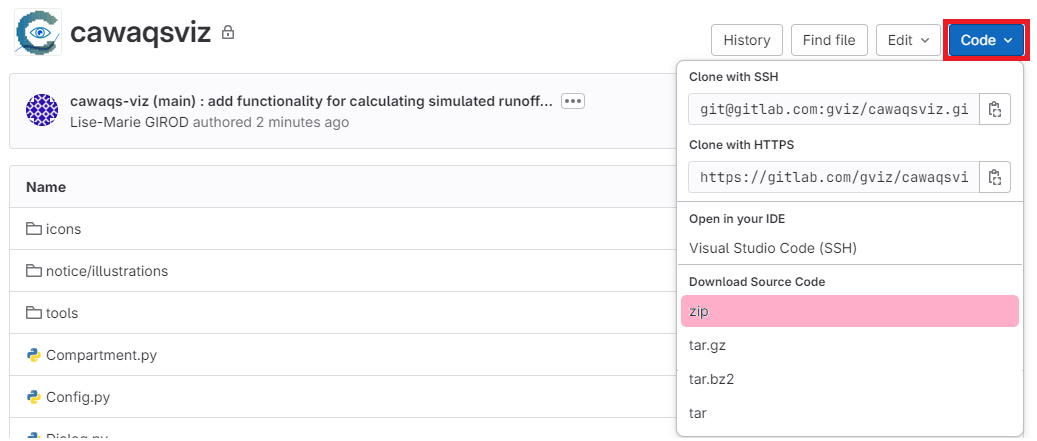
\includegraphics[width=0.8\linewidth]{1_installation_requirements/fig/download_gitlab.png}
    \caption{Téléchargement de l'archive \cwv~depuis l'interface web de dépôt \gitlab.}
    \label{fig-download_cwv}
\end{figure}

Dans la barre supérieure de menus de QGIS, cliquez sur \gui{Extensions} puis \gui{Installer/Gérer les extensions}. La fenêtre de gestion et d'import des extensions s'ouvre. Sélectionner \gui{Installer depuis un ZIP} (\cref{fig-QGIS_install_from_zip}). 

\begin{figure}[H]
    \centering
    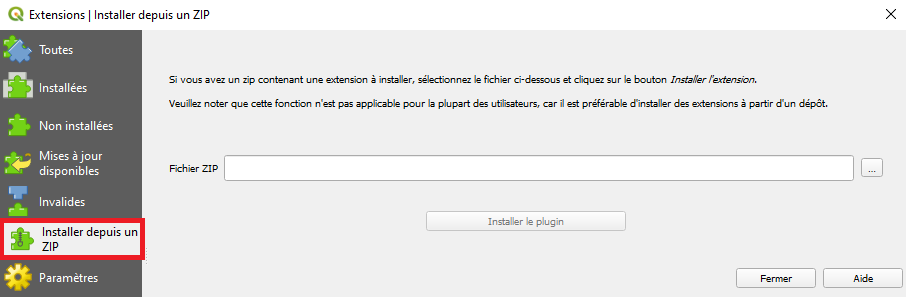
\includegraphics[width=1\linewidth]{1_installation_requirements/fig/QGIS_install_from_zip.png}
    \caption{Boîte de dialogue QGIS pour la gestion d'extensions.}
    \label{fig-QGIS_install_from_zip}
\end{figure}

Une fois le fichier \script{.zip} décompressé sous QGIS, il peut être nécessaire d'activer ce dernier dans la même fenêtre de gestion des extensions en naviguant dans le volet \gui{Installées}. L'extension \cwv~doit être cochée pour figurer dans la barre d'outils QGIS (\cref{fig-CWV-activation}).

\begin{figure}[H]
    \centering
    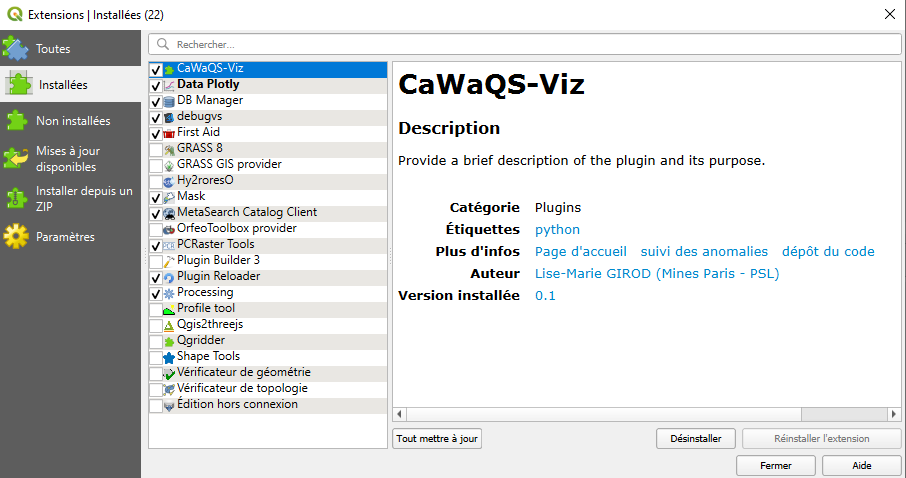
\includegraphics[width=1\linewidth]{couverture/fig/QGIS_get_plugin_in_toolbar.png}
    \caption{Activation de l'extension \cwv~dans l'application QGIS.}
    \label{fig-CWV-activation}
\end{figure}

Une fois l'application présente dans la barre d'outils de QGIS, celle-ci est prête à être lancée d'un simple clic sur l'icône 
\includegraphics[height=0.45cm]{couverture/fig/Icon_CaWaQSVIZ.png}.

\alertinfo{Pour utiliser toute nouvelle mise à jour du plug-in dans QGIS, il sera nécessaire de réitérer l'intégralité de cette procédure (\cref{sec-install-user}).}

\section{Installation pour les développeurs} \label{sec-install-expert}

Le répertoire de dépôt \gitlab~de \cwv~peut être cloné depuis un terminal de commande : 

\begin{lstlisting}[language=bash]
$ git clone https://gitlab.com/gviz/cawaqsviz
\end{lstlisting}

Le répertoire de l'application doit être placer à l'emplacement (dossier) des applications natives de QGIS afin que toute modification du code source du plug-in puisse être prise en compte par QGIS lors de son démarrage. Le répertoire QGIS est accessible \textit{via} le chemin suivant :

\begin{lstlisting}[language=bash]
#windows
C:/Programmes/QGIS3.X.X.X/apps/qgis-ltr/python/plugin/
#linux 
/home/bin/QGIS3.X.X.X/apps/qgis-ltr/python/plugin/
\end{lstlisting}


La structure du code du plug-in est décrite en chapitre \ref{chap-description-src}.\\

\alertinfo{L'autocomplétion des fonctionnalités liées à la libraire qgis est diponible à condition d'utiliser l'interpréteur python utilisé par QGIS. Un environnement virutel peut-être initalisé à cet effet.}

\textbf{N.B.} : Pour faciliter le développement du plug-in, les utilitaires suivants peuvent être installés depuis le gestionnaire des applications QGIS :
\begin{enumerate}
    \item \textbf{Reloader} permet de recharger le plug-in sans relancer QGIS à chaque modification de code, 
    \item \textbf{FirstAid} permet une visualisation détaillée des erreurs retournées par l'interpréteur Python de QGIS ainsi que les différents objets et variables liées à l'extension. 
\end{enumerate}

